\usepackage{tikz}
\usepackage{tcolorbox}

\definecolor{coverblue}{RGB}{0,70,150}
\definecolor{coverdarkblue}{RGB}{0,40,100}
\definecolor{accentgreen}{RGB}{74,222,128}

\renewcommand{\maketitle}{
  \begin{titlepage}
    \thispagestyle{empty}
    \begin{tikzpicture}[remember picture, overlay]
      % Bloque azul en la parte superior (~62% de la pagina)
      \fill[coverblue] (current page.north west) rectangle
        ([yshift=-0.62\paperheight]current page.north east);

      % ===== Titulo (marca) en Georgia bold =====
      \node[anchor=center, text=white, font=\Huge\bfseries, align=center, text width=0.9\paperwidth]
        at ([yshift=-0.085\paperheight]current page.north)
        {Aprende Java\\[0.18em]Jugando};

      % ===== Mockup de la ventana del juego (imagen central) =====
      \node[anchor=center] at ([yshift=-0.335\paperheight]current page.north)
        {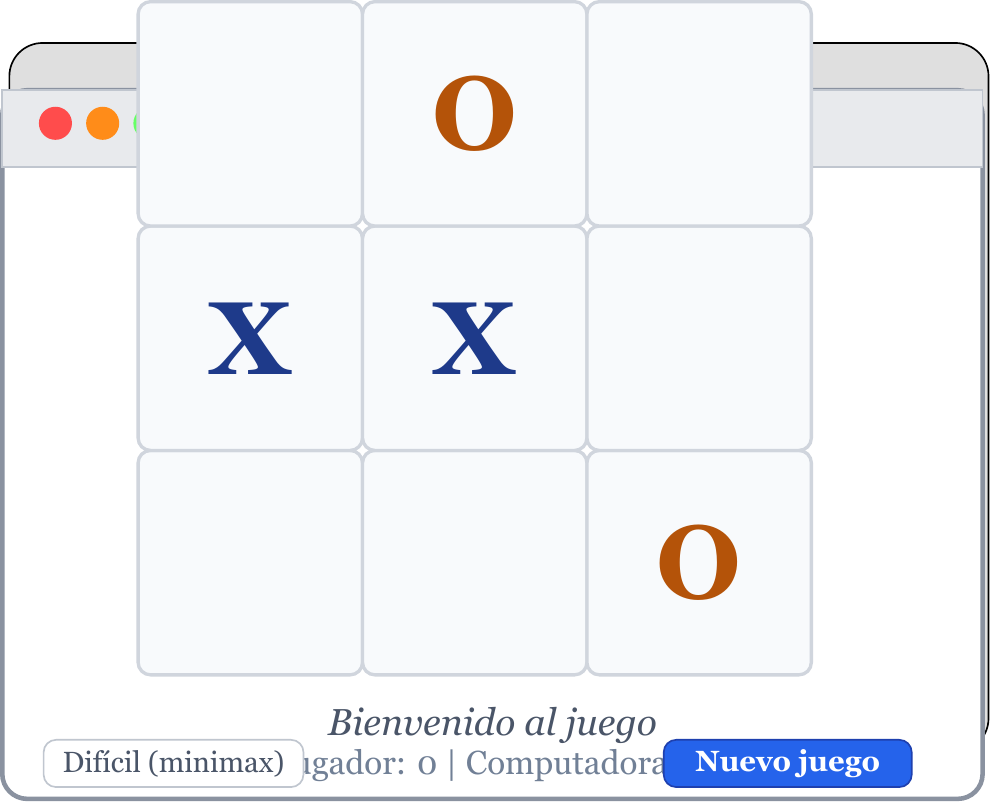
\includegraphics[width=0.415\paperwidth]{assets/mockup_juego.png}};

      % ===== Subtitulo de venta, dentro del bloque azul, acento verde =====
      \node[anchor=center, text=white, font=\Large, align=center, text width=0.8\paperwidth]
        at ([yshift=-0.555\paperheight]current page.north)
        {De no saber programar a tu primer juego\\con \textcolor{accentgreen}{\textbf{Inteligencia Artificial}} (Minimax)};

      % ===== Autor en azul oscuro, debajo del bloque =====
      \node[anchor=center, text=coverdarkblue, font=\large, align=center]
        at ([yshift=-0.74\paperheight]current page.north)
        {Carlos Alberto Robayo Delgado};

      % ===== Linea de credibilidad en gris =====
      \node[anchor=center, text=gray, font=\large, align=center]
        at ([yshift=-0.80\paperheight]current page.north)
        {Curso práctico, guiado y con retos de código};

      % Linea decorativa azul en la parte inferior
      \fill[coverblue] ([yshift=1.5cm]current page.south west) rectangle
        ([yshift=1.65cm]current page.south east);
    \end{tikzpicture}
  \end{titlepage}
}